\documentclass[11pt,a4paper]{article}
\usepackage[utf8]{inputenc}
\usepackage[T1]{fontenc}
\usepackage[french]{babel}
\usepackage{amsmath,amssymb}
\usepackage{geometry}
\usepackage{fancyhdr}
\usepackage{enumitem}
\usepackage{multicol}
\usepackage{tikz}
\usetikzlibrary{calc,arrows.meta,shapes.geometric,positioning,backgrounds}
\usepackage{pgfplots}
\pgfplotsset{compat=1.18}
\usepackage{xcolor}
\usepackage{graphicx}
\usepackage{array}
\usepackage{fontawesome5}
\usepackage{tabularx}
\usepackage[most]{tcolorbox}
\usepackage{wrapfig}

% Définition des couleurs modernes
\definecolor{primary}{RGB}{41, 128, 185}      % Bleu moderne
\definecolor{secondary}{RGB}{52, 73, 94}      % Gris foncé
\definecolor{accent}{RGB}{46, 204, 113}       % Vert menthe
\definecolor{warning}{RGB}{231, 76, 60}       % Rouge moderne
\definecolor{light}{RGB}{236, 240, 241}       % Gris très clair
\definecolor{bglight}{RGB}{247, 249, 250}     % Fond clair

\DeclareRobustCommand{\rep}[1]{\begingroup\color{warning}\ifmmode #1\else \textbf{#1}\fi\endgroup}

% Configuration de la page
\geometry{
	top=1.5cm,
	bottom=2cm,
	left=1.8cm,
	right=1.8cm
}

% Configuration tcolorbox
\tcbuselibrary{skins,breakable}

% Boîte pour les exercices
\newtcolorbox{exercisebox}[2][]{
	colback=white,
	colframe=primary,
	fonttitle=\bfseries\large,
	title={#2},
	arc=2mm,
	boxrule=1.5pt,
	left=15pt,
	right=15pt,
	top=12pt,
	bottom=12pt,
	boxsep=0pt,
	breakable,
	enhanced,
	width=\linewidth,
	grow to left by=3mm,
	grow to right by=3mm,
	#1
}

% Boîte pour les consignes
\newtcolorbox{consignebox}{
	colback=light!30,
	colframe=secondary,
	arc=3mm,
	boxrule=0pt,
	leftrule=4pt,
	left=15pt,
	right=15pt,
	top=12pt,
	bottom=12pt,
	enhanced,
	width=\linewidth,
	grow to left by=3mm,
	grow to right by=3mm
}

% En-tête et pied de page personnalisés
\pagestyle{fancy}
\fancyhf{}
\fancyhead[L]{\color{secondary}\textbf{5\textsuperscript{e}} | Mathématiques}
\fancyhead[R]{\color{secondary}\textbf{Symétrie centrale}}
\fancyfoot[C]{\color{secondary}\thepage}
\renewcommand{\headrulewidth}{0pt}
\renewcommand{\footrulewidth}{0pt}

% Commandes personnalisées
\newcommand{\points}[1]{\hfill \colorbox{primary}{\color{white}\textbf{\,#1 pts\,}}}
\newcommand{\badge}[2]{\tikz[baseline=(char.base)]{\node[shape=rectangle,draw,thick,rounded corners=2mm,inner sep=2pt,fill=#1,text=white,font=\footnotesize\bfseries] (char) {#2};}}

% Pointillés et zones de réponse
\newcommand{\dotline}[1]{\makebox[#1][s]{\dotfill}}
\newcolumntype{L}[1]{>{\hsize=#1\hsize\arraybackslash}X}

\begin{document}

	% En-tête moderne avec TikZ
	\begin{tikzpicture}[remember picture,overlay]
		\fill[primary] (current page.north west) rectangle ([yshift=-3.5cm]current page.north east);
		\node[anchor=north west,text=white,font=\Huge\bfseries] at ([xshift=2cm,yshift=-1cm]current page.north west) {Contrôle \no 2};
		\node[anchor=north west,text=white,font=\Large] at ([xshift=2cm,yshift=-2cm]current page.north west) {Symétrie centrale};
		\node[anchor=north east,text=white,font=\large] at ([xshift=-2cm,yshift=-1.5cm]current page.north east) {\faIcon{clock} 55 minutes};
		\node[anchor=north east,text=white,font=\large] at ([xshift=-2cm,yshift=-2.3cm]current page.north east) {\faIcon{calculator} Calculatrice non autorisée};
	\end{tikzpicture}

	\vspace{1.5cm}

	% Informations élève
	\begin{tcolorbox}[
		colback=bglight,colframe=secondary,arc=3mm,boxrule=1pt,
		left=15pt,right=15pt,top=10pt,bottom=10pt,
		enhanced,
		width=\linewidth,
		grow to left by=5mm,
		grow to right by=5mm
		]
		\setlength{\tabcolsep}{4pt}
		\begin{tabularx}{\linewidth}{@{}lX lX l@{}}
			\multicolumn{2}{@{}l}{\faIcon{user} \textbf{NOM :} \dotline{6cm}} &
			\multicolumn{2}{l@{}}{\textbf{Prénom :} \dotline{3cm}} &
			\\[0.5cm]
			\textbf{Classe :} & \dotfill &
			\faIcon{calendar} \textbf{Date :} & \dotfill &
			\fcolorbox{secondary}{white}{\textbf{NOTE : }\makebox[1.4cm]{\rule{0pt}{1.1em}}\textbf{ / 20}}
		\end{tabularx}
	\end{tcolorbox}

	\vspace{0.2cm}

	% Barème
	\begin{center}
		\badge{primary}{Ex.1: 5pts} \quad
		\badge{primary}{Ex.2: 3pts} \quad
		\badge{primary}{Ex.3: 4pts} \quad
		\badge{primary}{Ex.4: 4pts} \quad
		\badge{primary}{Ex.5: 4pts}
	\end{center}

	\vspace{0.2cm}

	% Consignes
	\begin{consignebox}
		\faIcon{info-circle} \textbf{CONSIGNES IMPORTANTES}
		\begin{itemize}[leftmargin=*,noitemsep,topsep=5pt]
			\item[\faIcon{check}] Répondez sur votre copie pour les exercices de construction
			\item[\faIcon{check}] Utilisez le matériel de géométrie (règle, compas, ...)
			\item[\faIcon{check}] Justifiez vos réponses quand c'est demandé
			\item[\faIcon{pencil-alt}] Écrivez lisiblement
		\end{itemize}
	\end{consignebox}

	\vspace{0.3cm}

	% Exercice 1
	\begin{exercisebox}{\faIcon{search} Exercice 1 : Reconnaître des symétriques \points{5}}

		\begin{minipage}[c]{0.35\linewidth}
			\centering
			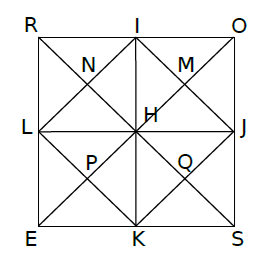
\includegraphics[width=\linewidth]{images_controle_2/fig_1_ex_1}
		\end{minipage}%
		\hfill
		\begin{minipage}[c]{0.62\linewidth}
			\begin{enumerate}[label=\textcolor{primary}{\textbf{\alph*)}},leftmargin=*,topsep=0pt]
				\item Quel est le symétrique du triangle $RNI$ par rapport au point $N$ ? \points{1}

				\vspace{0.2cm}

				\item Quel est le symétrique du triangle $HMJ$ par rapport au point $H$ ? \points{1}

				\vspace{0.3cm}

				\item Quel est le symétrique du triangle $JQS$ par rapport au point $Q$ ? \points{1}

				\vspace{0.3cm}

				\item Colorie en rouge le symétrique du triangle $OJM$ par rapport à $H$. \points{1}

				\vspace{0.2cm}

				\item Colorie en bleu le symétrique du triangle $HIR$ par rapport à $H$. \points{1}
			\end{enumerate}
		\end{minipage}
	\end{exercisebox}

	\vspace{0.2cm}

	% Exercice 2
		\begin{exercisebox}{\faIcon{font} Exercice 2 : Symétrie de lettres \points{3}}
		
		\begin{minipage}[c]{0.45\linewidth}
			\centering
			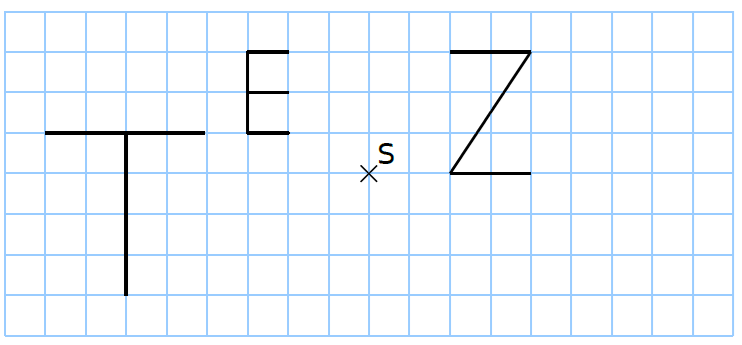
\includegraphics[width=\linewidth]{images_controle_2/fig_1_ex_2}
		\end{minipage}%
		\hfill
		\begin{minipage}[c]{0.52\linewidth}
			Construis le symétrique de chaque lettre par rapport au point $S$.
		\end{minipage}
	\end{exercisebox}
	
	
	\vspace{0.3cm}

	% Exercice 3

\begin{exercisebox}{\faIcon{drafting-compass} Exercice 3 : Construction de symétriques \points{4}}
	
	\begin{minipage}[c]{0.35\linewidth}
		\centering
		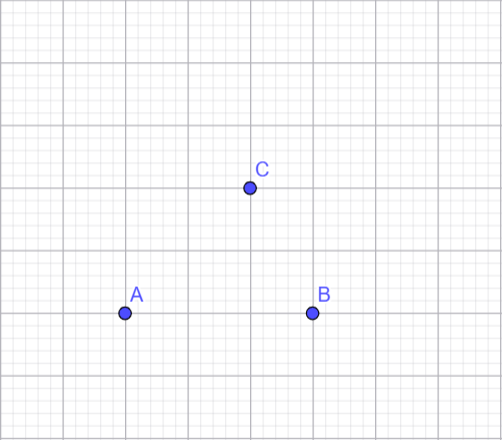
\includegraphics[width=\linewidth]{images_controle_2/fig_1_ex_3}
	\end{minipage}%
	\hfill
	\begin{minipage}[c]{0.62\linewidth}
		\begin{enumerate}[label=\textcolor{primary}{\textbf{\alph*)}},leftmargin=*,topsep=0pt]
			\item Construis le point $D$, symétrique du point $B$ par rapport à $C$. \points{1}
			
			\vspace{0.2cm}
			
			\item Construis le point $E$, symétrique du point $A$ par rapport à $C$. \points{1}
			
			\vspace{0.2cm}
			
			\item Quel est le symétrique du triangle $ABC$ par rapport à $C$ ? \points{1}
			
			\vspace{0.2cm}
			
			\item Construis en vert le symétrique du triangle $ABC$ par rapport à $B$. \points{1}
		\end{enumerate}
	\end{minipage}
\end{exercisebox}

	\vspace{0.2cm}

	% Exercice 4
	\begin{exercisebox}{\faIcon{shapes} Exercice 4 : Construction avec instruments \points{4}}

		\begin{minipage}[c]{0.60\linewidth}
			\centering
			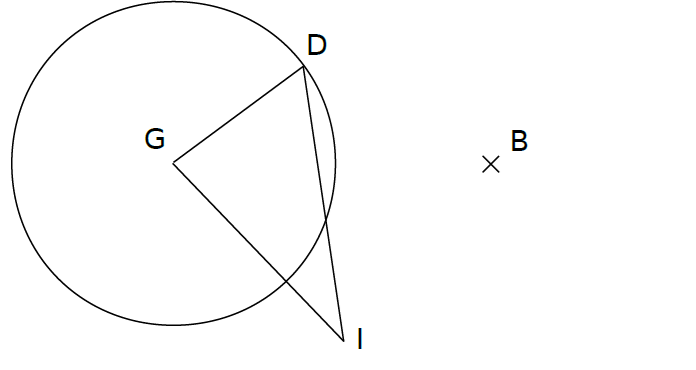
\includegraphics[width=0.8\linewidth]{images_controle_2/fig_1_ex_4}
		\end{minipage}%
		\hfill
		\begin{minipage}[c]{0.4\linewidth}
			Construis, avec tes instruments, le symétrique de la figure ci-contre par rapport au point $B$.
		\end{minipage}
	\end{exercisebox}

	\vspace{0.2cm}

	% Exercice 5
	\begin{exercisebox}{\faIcon{star} Exercice 5 : Propriétés de la symétrie centrale \points{4}}

		\begin{minipage}[t]{0.35\linewidth}
			\centering
			\vspace{0.3cm}
			$U$ est un centre de symétrie de la figure ci-contre.

			\vspace{0.3cm}
			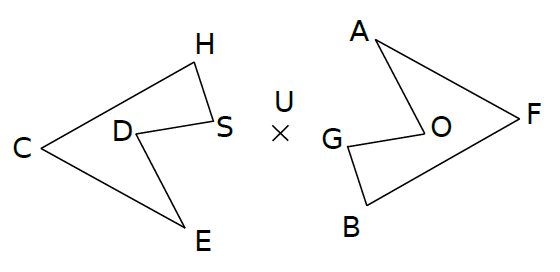
\includegraphics[width=\linewidth]{images_controle_2/fig_1_ex_5}
		\end{minipage}%
		\hfill
		\begin{minipage}[t]{0.62\linewidth}
			\begin{enumerate}[label=\textcolor{primary}{\textbf{\alph*)}},leftmargin=*,topsep=0pt]
				\item Quel est le symétrique du point $D$ par rapport à $U$ ? \points{1}

				\vspace{0.2cm}

				\item Quel segment a la même longueur que $[AF]$ ? Pourquoi ? \points{1}

				\vspace{0.5cm}

				\item Quelle droite est parallèle à $(HS)$ ? Pourquoi ? \points{1}

				\vspace{0.5cm}

				\item Quel angle a la même mesure que l'angle $\widehat{DEC}$ ? Pourquoi ? \points{1}
			\end{enumerate}
		\end{minipage}
	\end{exercisebox}

	% Pied de page avec évaluation
	\vspace{0.3cm}
	\begin{center}
		\begin{tikzpicture}
			\node[draw=secondary,rounded corners=3mm,inner sep=8pt,fill=light!30] {
				\begin{tabular}{lccccc}
					\textbf{Auto-évaluation :} &
					\faIcon{frown} Difficile &
					\faIcon{meh} Moyen &
					\faIcon{smile} Facile &
					\phantom{xx} &
					\textbf{Temps utilisé :} \underline{\phantom{xxxxx}} min
				\end{tabular}
			};
		\end{tikzpicture}
	\end{center}

	\newpage

	% =======================
	% CORRIGÉ
	% =======================

	\begin{center}
		\Large\textbf{\color{warning}CORRIGÉ}
	\end{center}

	\vspace{0.5cm}

	% Exercice 1 - Corrigé
	\begin{exercisebox}{\faIcon{search} Exercice 1 — Corrigé}
		\begin{minipage}[c]{0.25\linewidth}
			\begin{center}
				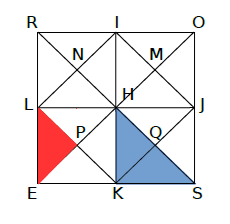
\includegraphics[width=0.8\linewidth]{images_controle_2/fig_1_ex_1_correction}
			\end{center}
			
		\end{minipage}%
		\hfill
		\begin{minipage}[c]{0.75\linewidth}
			\begin{enumerate}[label=\textcolor{primary}{\textbf{\alph*)}},leftmargin=*,topsep=0pt]
				\item \rep{NLH} est le symétrique du triangle $RNI$ par rapport au point $N$.

				\item \rep{HLP} est le symétrique du triangle $HMJ$ par rapport au point $H$.

				\item \rep{HQK} est le symétrique du triangle $JQS$ par rapport au point $Q$.

				\item Le triangle rouge (symétrique de $OJM$ par rapport à $H$) est \rep{EKP}.

				\item Le triangle bleu (symétrique de $HIR$ par rapport à $H$) est \rep{KQS}.
			\end{enumerate}
		\end{minipage}
	\end{exercisebox}

	\vspace{0.3cm}

	% Exercice 2 - Corrigé
	\begin{exercisebox}{\faIcon{drafting-compass} Exercice 2 — Corrigé}
		\begin{minipage}[c]{0.40\linewidth}
			\begin{center}
				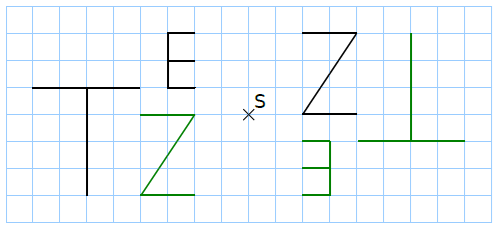
\includegraphics[width=0.7\linewidth]{images_controle_2/fig_1_ex_2_correction}
			\end{center}
			
		\end{minipage}%
		\hfill
		\begin{minipage}[c]{0.52\linewidth}
			Pour chaque point de chaque lettre, construire son symétrique par rapport à $S$ :
			\begin{itemize}[leftmargin=*]
				\item Tracer la droite passant par le point et $S$
				\item Reporter la distance de l'autre côté de $S$
				\item Relier les points images pour former les lettres symétriques
			\end{itemize}
		\end{minipage}
	\end{exercisebox}

	\vspace{0.2cm}

	% Exercice 3 - Corrigé
	\begin{exercisebox}{\faIcon{font} Exercice 3 — Corrigé}
		\begin{minipage}[c]{0.45\linewidth}
			\begin{center}
				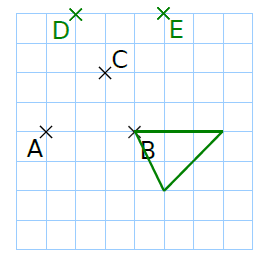
\includegraphics[width=0.7\linewidth]{images_controle_2/fig_1_ex_3_correction}
			\end{center}
			
		\end{minipage}%
		\hfill
		\begin{minipage}[c]{0.57\linewidth}
			\begin{enumerate}[label=\textcolor{primary}{\textbf{\alph*)}},leftmargin=*,topsep=0pt]
				\item Construction du point $D$ : tracer la droite $(BC)$, prolonger au-delà de $C$, reporter la distance $BC$ pour obtenir $D$ tel que $C$ soit le milieu de $[BD]$.
				
				\item Construction du point $E$ : tracer la droite $(AC)$, prolonger au-delà de $C$, reporter la distance $AC$ pour obtenir $E$ tel que $C$ soit le milieu de $[AE]$.
				
				\item \rep{CDE} est le symétrique du triangle $ABC$ par rapport à $C$.
				
				\item Construire les images de $A$ et $C$ par la symétrie de centre $B$ pour obtenir le triangle symétrique en vert.
			\end{enumerate}
		\end{minipage}
	\end{exercisebox}

	\vspace{0.3cm}

	% Exercice 4 - Corrigé
	\begin{exercisebox}{\faIcon{shapes} Exercice 4 — Corrigé}
		\begin{minipage}[c]{0.50\linewidth}
			\begin{center}
				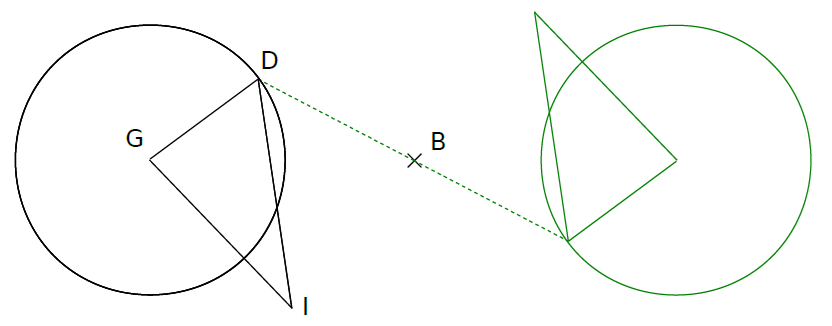
\includegraphics[width=0.8\linewidth]{images_controle_2/fig_1_ex_4_correction}
			\end{center}
			
		\end{minipage}%
		\hfill
		\begin{minipage}[c]{0.5\linewidth}
			Pour construire le symétrique :
			\begin{itemize}[leftmargin=*]
				\item Construire les images des points $G$, $D$ et $I$ par la symétrie de centre $B$
				\item Le cercle symétrique a pour centre l'image de $G$ et le même rayon
				\item Tracer le triangle avec les images des points
			\end{itemize}
		\end{minipage}
	\end{exercisebox}

	\vspace{0.3cm}

	% Exercice 5 - Corrigé
	\begin{exercisebox}{\faIcon{star} Exercice 5 — Corrigé}
		\begin{enumerate}[label=\textcolor{primary}{\textbf{\alph*)}},leftmargin=*]
			\item \rep{O} est le symétrique du point $D$ par rapport à $U$.

			\item \rep{[CE]} est le symétrique de $[AF]$ par rapport à $U$.

			Comme la symétrie centrale conserve les longueurs, \rep{$AF = CE$}.

			\item \rep{(GB)} est le symétrique de $(HS)$ par rapport à $U$.

			Comme la symétrie centrale transforme une droite en une droite parallèle, alors \rep{$(GB)$ et $(HS)$ sont parallèles}.

			\item \rep{$\widehat{FAO}$} est le symétrique de $\widehat{DEC}$ par rapport à $U$.

			Comme la symétrie centrale conserve les angles, \rep{$\widehat{FAO} = \widehat{DEC}$}.
		\end{enumerate}
		\begin{center}
			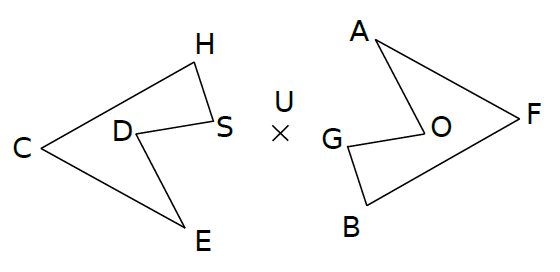
\includegraphics[width=0.5\linewidth]{images_controle_2/fig_1_ex_5}
		\end{center}
		
	\end{exercisebox}

\end{document}
